\chapter{Results}
%\section{Comparison to Theory}
%Add figure of Pion spectra for different theory 
%Reference paper for multiple theories

 The data taken has been compared with 7 commonly used transport theoretical codes. These codes took part in a large collaborative effort in order to standardize certain common elements of each codes \cite{theoryComp1,theoryComp2}. To reduce uncertainties in the pion production mechanism, each model used comparison project simulated nuclear matter in a box type simulation with fixed, well defined, initial conditions. Though these box calculations model an equilibrated system at finite density, which is  not replicated by experiment, the limit is theoretically clearly defined and provides a benchmark comparison between models where the solutions  yield values for the total number of produced pions and $\Delta$ that can be analytically calculated from the ansatz of  statistical equilibrium, providing a good benchmark. This allowed for each code to systematically go through the numerical treatment and details in each code such as initialization of nuclei, stability of the code, numerical handing of pauli-blocking, etc. After satisfying these benchmark calculations, each model was used with what the authors considered the most reliable input and model assumption.  codes were taken in their best configuration, as a result of these comparison projects, without any prior knowledge of the experimental data. We then simulated the 4 systems measured in the \spirit TPC at an impact parameter of \SI{3}{\femto\metre} at \SI{270}{\MeVA} beam energy. While the numerical treatments of each code are reasonably similar, each code differs considerably in their treatment of pion and $\Delta$ dynamics. Some codes contain modifications to how the pion behaves in nuclear matter, i.e. \emph{in-medium effects}, typically introduced by including a pion optical potential which describes the pion scattering and absorption. Some codes include the iso-scalar and the iso-vector delta potential, which are not very well constrained but can be important in the production of pions \cite{baoan_deltapotential,inmedPionKo,inmedPionFeng}. The set of 7 codes represent the best codes at the moment, which can simulate pions at these energies. 


It is important to note that the interaction of pions and deltas with dense matter should not be viewed as a nasty detail that a "better" probe like nucleonic elliptical flow would avoid. One of the central questions regarding matter at twice saturation density concerns the importance of deltas and pions as important constituents of the matter at those densities \cite{pionNS,deltaNS,awayforward}. Questions of the role of delta's and pion at 2$\rho_o$ are strongly connect to these potentials. Calculations of pion production indicate that selected pionic observables such as the energy spectra and transverse momentum distributions can be used to constrain these densities \cite{cozmaPC}. Obtaining such constraints are a major objective of our current work, but such constraints are ready for discussion at the present time. 

As will be the re-occurring theme, there is a large variation in the predicted observables, between theoretical codes; greater than the variation between different symmetry energy in a particular code. However, the remedy for this discrepancy is for the authors of these models to include the other physics that many of them have neglected. This includes a better description of delta interactions of matter, which is critical to reproducing the total pion yields, and also the momentum dependence of the isovector mean field potentials, which have a large impact on the shapes of the energy spectra. Though some of the elementary issues relevant to such transport theories, such as the Pauli principal and the incorporation of inelastic processes, have been addressed. The relevant physics include the mean field potentials for nucleons, pions and deltas. A primary focus is on the isovector potentials of which only the momentum independent potentials for nucleons have been varied in the calculations shown below. The momentum dependent nucleonic mean field potentials and the mean field potentials for delta's and pions are only included in a subset of calculations. Calculations have already identified that the overall pion yield are influenced by the mean field potentials for the delta's \cite{cozmaPC}, which may not be surprising since a similar sensitivity has govern the occurrence of for delta and pionic matter within neutron stars \cite{deltaNS,pionNS}.  

%Similar to the experience with the symmetric matter EoS, the next steps will be to connect these mean field to to observables and begin constraining them [cite danielewics science article and Cozma private communication] 
With the \spirit TPC, we were able to measure the pion yield without resorting to extrapolations, and were able to measure the pion energy spectra of low to high energy pions with high inefficiencies. In the following pages we will present the total pion yield and energy spectra of this dissertation, which complements the dissertaion of Jon Barney \cite{jon}.


%to provide much needed experimental data in which each code may compare too. The total theoretical uncertainty is too large relative to the experimental error bars to make a constraint on the density dependence of the symmetry energy. Any constraint would depend on the particular code one is using and would result in conflicting conclusions when using another theory. There is no good consensus at this time which codes should be favored over other codes, as the magnitude of the effects included in each code are still debated in order of importance. Here I will present the current level of agreement with the codes and remark on some of the implications it has moving forward. 


\section{Pion Yield}

We begin with the total charged pion multiplicities for the two systems of extreme isospin asymmetry:  the neutron rich $\tin{132}{124}$ system and the neutron deficient  $\tin{108}{112}$ system. Though the previous FOPI data set provided significant constraints pertaining the the symmetry energy, they relied on extrapolations to low transverse momenta, $P_T = \sqrt{p_x^2 + p_y^2}$, below \SI{160}{\mega\electronvolt\per\clight} \cite{fopi}. In the \spirit TPC, we were able to measure pions to very low $P_T$ for rapidities $y > y{CM}$; where the rapidity is expressed along the beam direction (z) as,

\begin{equation}
y = \frac{1}{2} \ln\Big( \frac{E + p_zc}{E - p_zc}\Big).
\end{equation}

The pion rapidity in the COM system $y_{\pi CM}$ is normalized,

\begin{equation}
y_o = \frac{y_{\pi CM}}{y_{beam} - y_{CM}},
\end{equation}

where $y_{beam}$ is the beam rapidity in the lab frame and $y_{CM}$ is the CM system rapidity. This is keeping with the same notation of $y_o$ in Reference \cite{fopi}. Here $y_o = 1$ corresponds to a particle moving at beam rapidity. The   $P_T - y_o$ phase space of the \spirit TPC is plotted for both charged pions in the $\tin{132}{124}$ system , in Figure~\ref{ptrap_sn132}, and the $\tin{108}{112}$ system , in Figure~\ref{ptrap_sn108}. Good efficiency down to very low $P_T$ avoided any need for extrapolations. There was good acceptance of pions $y_o > 0$ -- corresponding to $\theta_{CM} < \ang{90}$ -- where we cut off the lower rapidities. This marks the first time that pions have been measured to such low $P_T$. 

\begin{figure}[!htb]
\centering
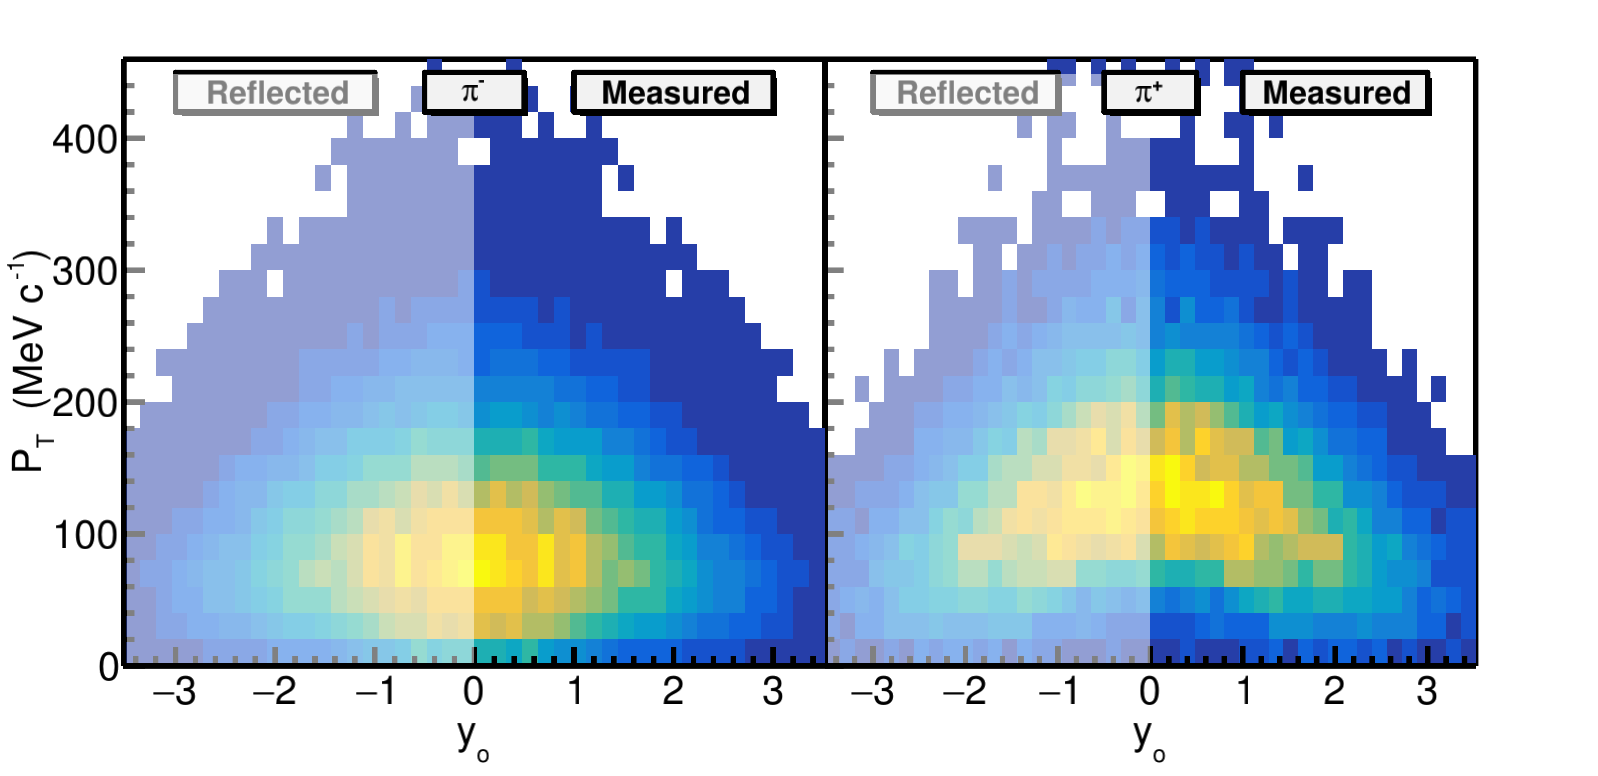
\includegraphics[width=\textwidth]{ypt_sn132.png}
\caption{Rapidity and transverse momentum plot for $\pi^-$ and $\pi^+$ in the $\tin{132}{124}$ system.}
\label{fig:ptrap_sn132}
\end{figure}


\begin{figure}[!htb]
\centering
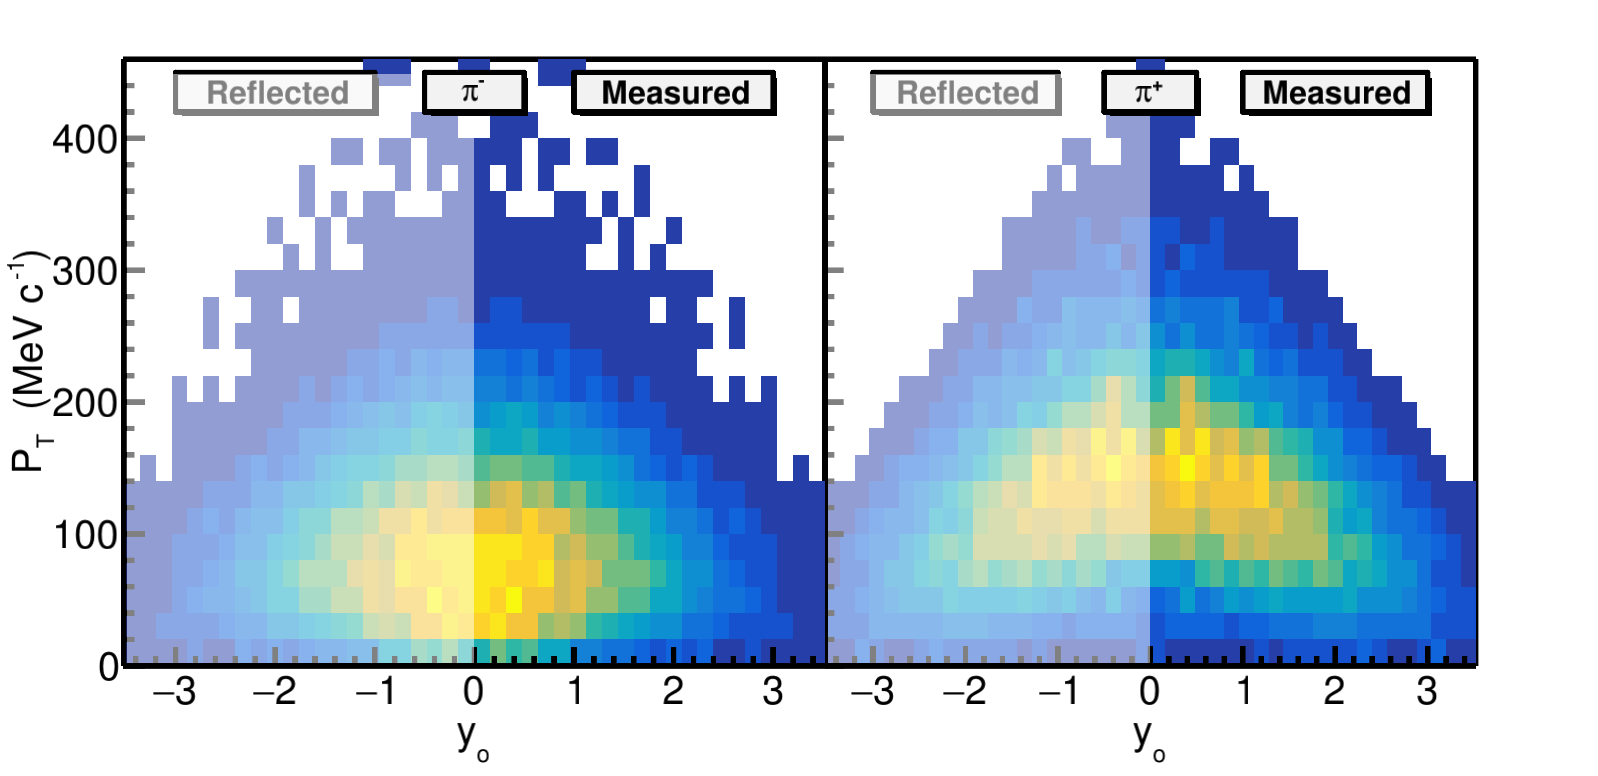
\includegraphics[width=\textwidth]{ypt_sn108.png}
\caption{Rapidity and transverse momentum plot for $\pi^-$ and $\pi^+$ in the $\tin{108}{112}$ system.}
\label{fig:ptrap_sn132}
\end{figure}

The integrated pion yield for both systems, and the $\pi^-/\pi^+$ ratio, is listed in Table~\ref{tb:pionyield}, where the systematic errors are the first error bar and the statistical error is listed next. Notice that the pion ratio is significantly greater than the $N/Z$ of the system.  This is not completely unexpected; in the Delta Resonance model where $\pi^-$ come primarily from neutron-neutron collisions and $\pi^+$ from proton-proton collisions, we expect  $\pi^-/\pi^+ = (N/Z)^2$ \cite{baoan_piprod1,baoan_piprod2}, where N/Z is the ratio of neutron to protons in the dense region where pions are produced. For the $\tin{132}{124}$ system $(N/Z)^2$ = 2.56 and for $\tin{108}{112}$ $(N/Z)^2$ = 1.44, but this naive scaling assumes no migration of nucleons in or out of the high density region where the isovector mean field and other transport properties may a impact that approximation significantly. 


Due to this connection between pion ratio and the isospin asymmetry at high density, the pion ratio was proposed to be a good probe of the isovector dynamics at high density. was hypothesized to be proportional to the high density N/Z ratio of the early system, where the other effects such as pion absorption and re-emission would dilute the effect, lowering the pion ratio as the system tends toward isospin equilibrium. It is likely however, that the dynamics plays are more significant role in pion productions via the $\Delta(1232)$ resonance than the simple $(N/Z)^2$ relation, which was also seen in \cite{fopi}. Some codes assume the potential of the delta is just the same as the corresponding nucleon potential, as given by the iso-spin. While other codes -- namly TuQMD -- introduce $\Delta$ resonance in-medium potential, which has an iso-scalar component (independent of iso-spin) and an iso-vector component.  The nature of these two potentials is still unknown, and the role it plays in pion production has shown to be very important \cite{baoan_deltapotential, cozmaPC}.


\begin{table*}\centering
\ra{1.3}
\begin{tabular}{@{}cccc@{}}\toprule
System & $\pi^-$ & $\pi^+$ & $Y(\pi^-)/Y(\pi^+)$  \\
\midrule
$\tin{132}{124}$ & 0.717(24)(4) & 0.148(5)(2) & 4.84(10)(6)  \\
$\tin{108}{112}$ & 0.399(14)(3) & 0.200(8)(2) & 1.99(4)(3)  \\
%$\tin{132}{124}$ & \numerr{0.717}{0.024}{0.004} & \numerr{0.148}{0.005}{0.002} & \numerr{4.84}{0.10}{0.06}  \\
%$\tin{108}{112}$ & \numerr{0.399}{0.014}{0.003} & \numerr{0.200}{0.008}{0.002} & \numerr{1.99}{0.04}{0.03}  \\
\bottomrule
\end{tabular}
\caption{Total pion yield.}
\label{tb:pionyield}
\end{table*}


We have compared the total pion yields and ratios to the 7 common transport codes for the systems measured. The table of the transport codes are listed in Appendix~\ref{tb:pionyieldTheory}. Figure~\ref{fig:totalpiYield} shows the total pion yield for the four systems measured as compared with the codes. The codes plotted here are only the soft symmetry energy since the variation in code is much larger than the variation within a code between different symmetry energies. While some codes make a reasonable approximation of a particular charge pion yields, no code reasonably predicts both. 

\begin{figure}[!htb]
\centering
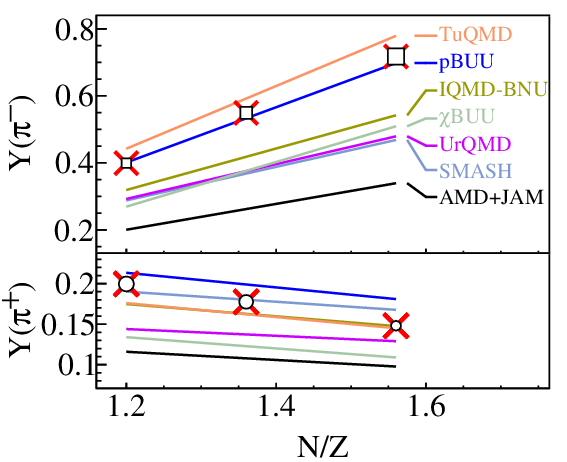
\includegraphics[width=.8\textwidth]{totalpiYield.png}
\caption{Total pion yields as compared with 7 common transport codes.}
\label{fig:totalpiYield}
\end{figure}

Figure~\ref{fig:totalpiRatio} shows the total single pion ratio, $R = Y(\pi^-)/Y(\pi^+)$, and the double ratio (DR), of the $\tin{132}{124}$ and $\tin{108}{112}$ system's single ratio, i.e. $DR = R_{\tin{132}{124}}/R_{\tin{124}{112}}$. Here, the variation between codes is much larger than the variation between the momentum dependence of the symmetry energy within a particular code. The symmetry energy variation (soft and stiff extremes) of two codes -- $\chi$BUU and TuQMD -- is plotted as a wide band in the single ratio and in all codes in the double ratio. The ciruclar markers and band represents the total error bar in the data. Certainly it can be seen that the variation between symmetry energy extremes in the codes, though small, still exists; as initially predicted \cite{baoan_piprod1,baoan_piprod2}, and the small error bars in the data would facilitate a detailed analysis to extract the high density behavior of the symmetry energy, if not for large disagreement between codes. 



\begin{figure}[!htb]
\centering
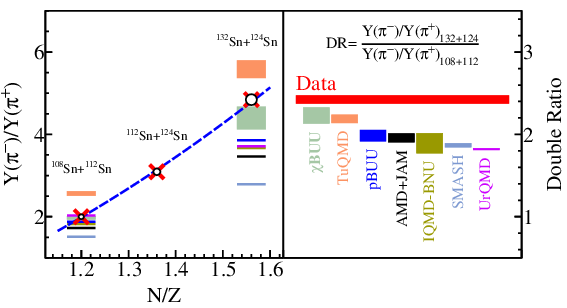
\includegraphics[width=\textwidth]{totalpiRatio.png}
\caption{Total pion ratio and double ratio compared with 7 common transport codes.}
\label{fig:totalpiRatio}
\end{figure}




\section{Comparison to Previous Data Sets (FOPI)}


\begin{figure}[!htb]
\centering
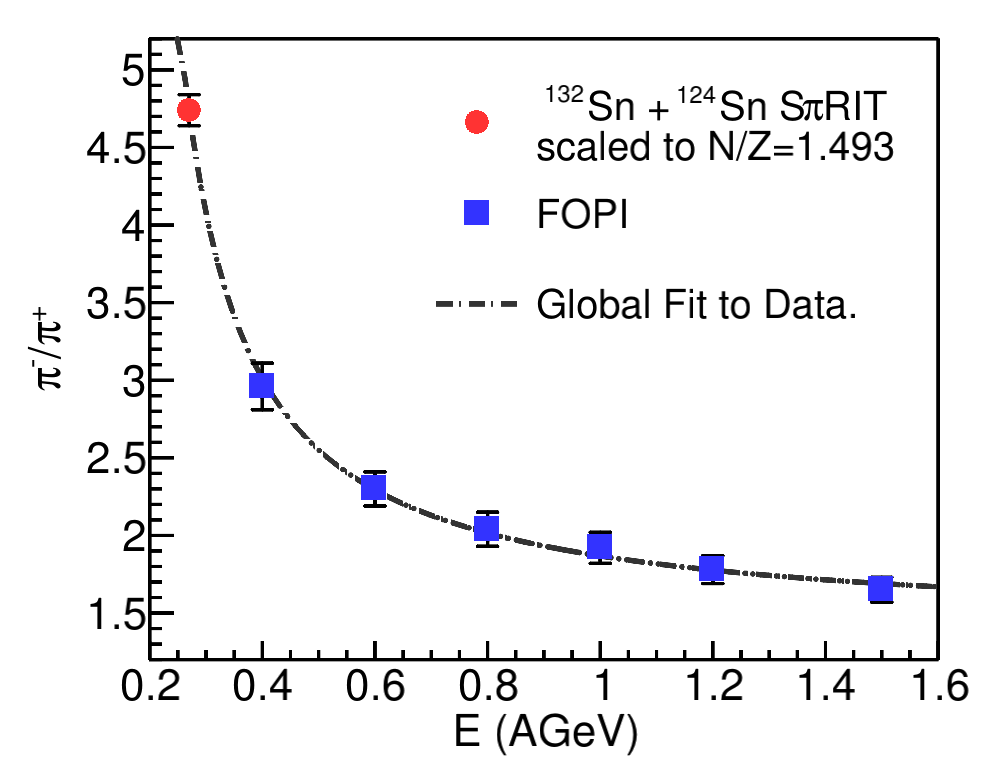
\includegraphics[scale=.4]{fopi_pionratio_comp}
\caption{Comparing the total $\pi^-/\pi^+$ ratio of the $\tin{132}{124}$ system to the ${}^{197}$Au + ${}^{197}$Au data from the FOPI collaboration. The \spirit TPC data was scaled by a factor to compare to the lower N/Z of the Au + Au system. This was extracted from measuring the N/Z dependence measured in the experiment. }
\label{fig:fopiPionRatio}
\end{figure}

The FOPI collaboration has measured the total pion multiplicity resulting from ${}^{197}Au + {}^{197}Au$ collisions at several, higher, beam energies. In the $\tin{132}{124}$ data the $N/Z=1.56$ where as in the ${}^{197}Au + {}^{197}Au$ the $N/Z=1.493$. We also expect the pion ratio is proportional to the $N/Z$ of the system. Since 4 beams were measured in this experiment, the $N/Z$ dependence was measured as seen in Fig.~\ref{fig:totalpiRatio}. Here the dependence is fitted with a 2-nd order polynomial fit. To compare the pion ratio in the $\tin{132}{124}$ data with that of the lower N/Z in the FOPI experiment, we scaled by the pion ratio between $N/Z=1.56$ and 1.493 as given from the fitted polynomial line. Figure~\ref{fig:fopiPionRatio} shows the scaled pion ratio as compared with the FOPI pion ratio \cite{fopi}. The fitted function has the functional form of $p_1(E - p_2)^{-2}$ where $p_1$ and $p_2$ are free parameters, and only is meant to guide the eye. It is also worth mentioning that the pion ratio observed in the FOPI \SI{400}{\MeVA} setting was already considerably higher than what is expected from the $(N/Z)^2$ delta resonance model \cite{baoan_piprod1,baoan_piprod2}. Scaling the other systems in the \spirit TPC data leads to almost the exact same value of $\mathrm{Y}(\pi^-)/\mathrm{Y}(\pi^+) = \num{4.82}$ and would be redundant. 




\section{Pion Spectra}
\label{sec:pionSpectra}



\begin{figure}[!htb]
\centering
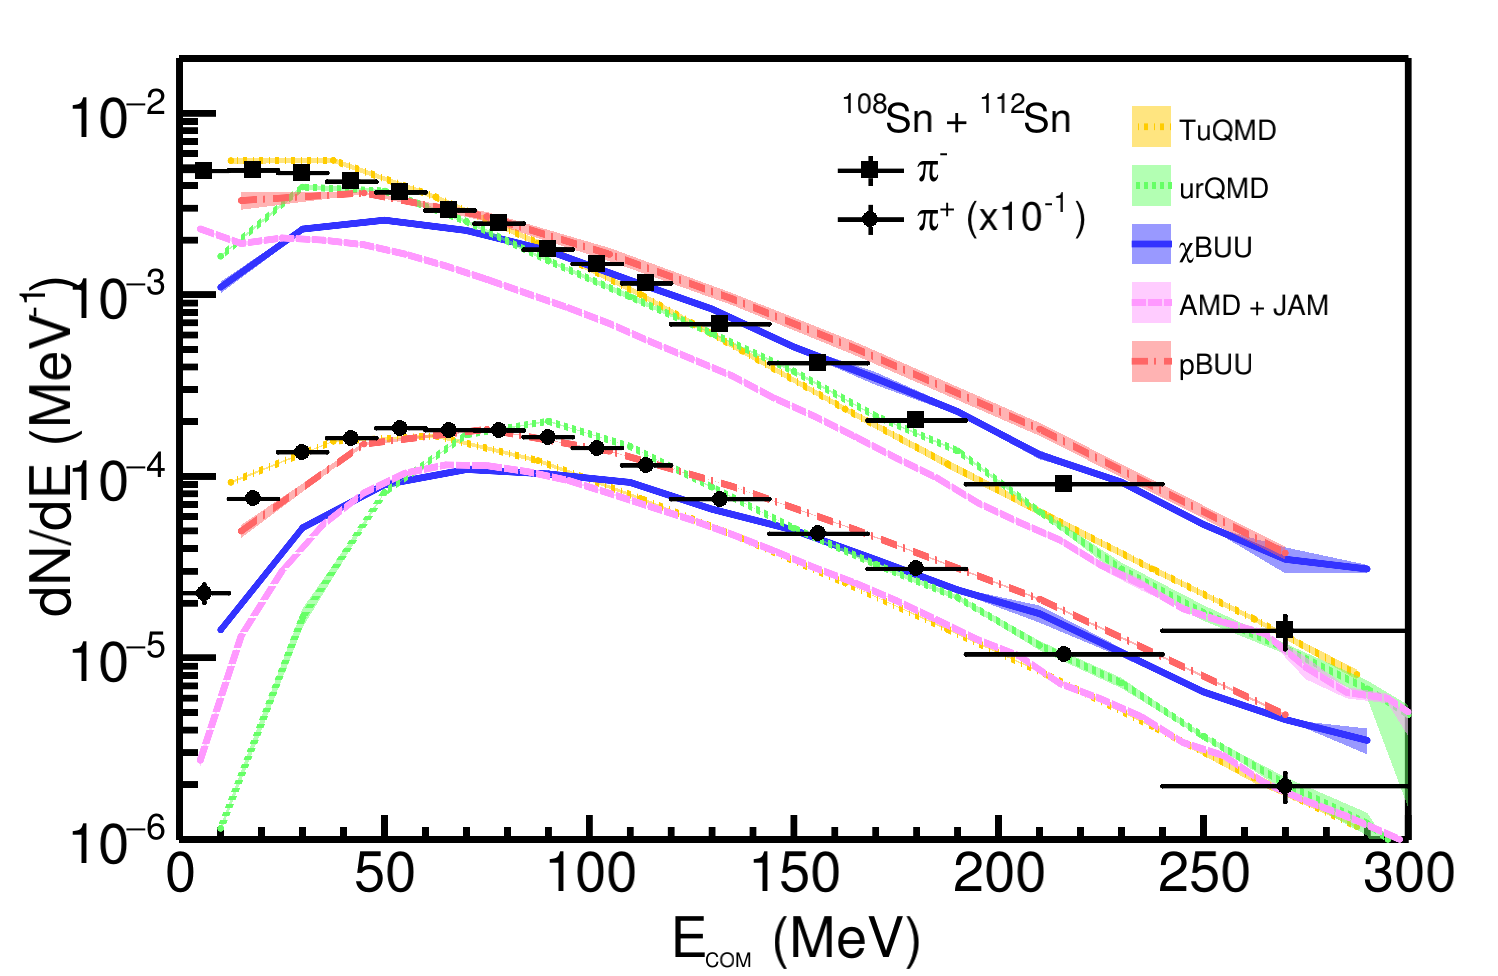
\includegraphics[width=\textwidth]{pionSpectra.png}
\caption{Pion spectra. }
\label{fig:pionspectra}
\end{figure}
%need to add error analysis
%systematic error analysis


\begin{figure}[!htb]
\centering
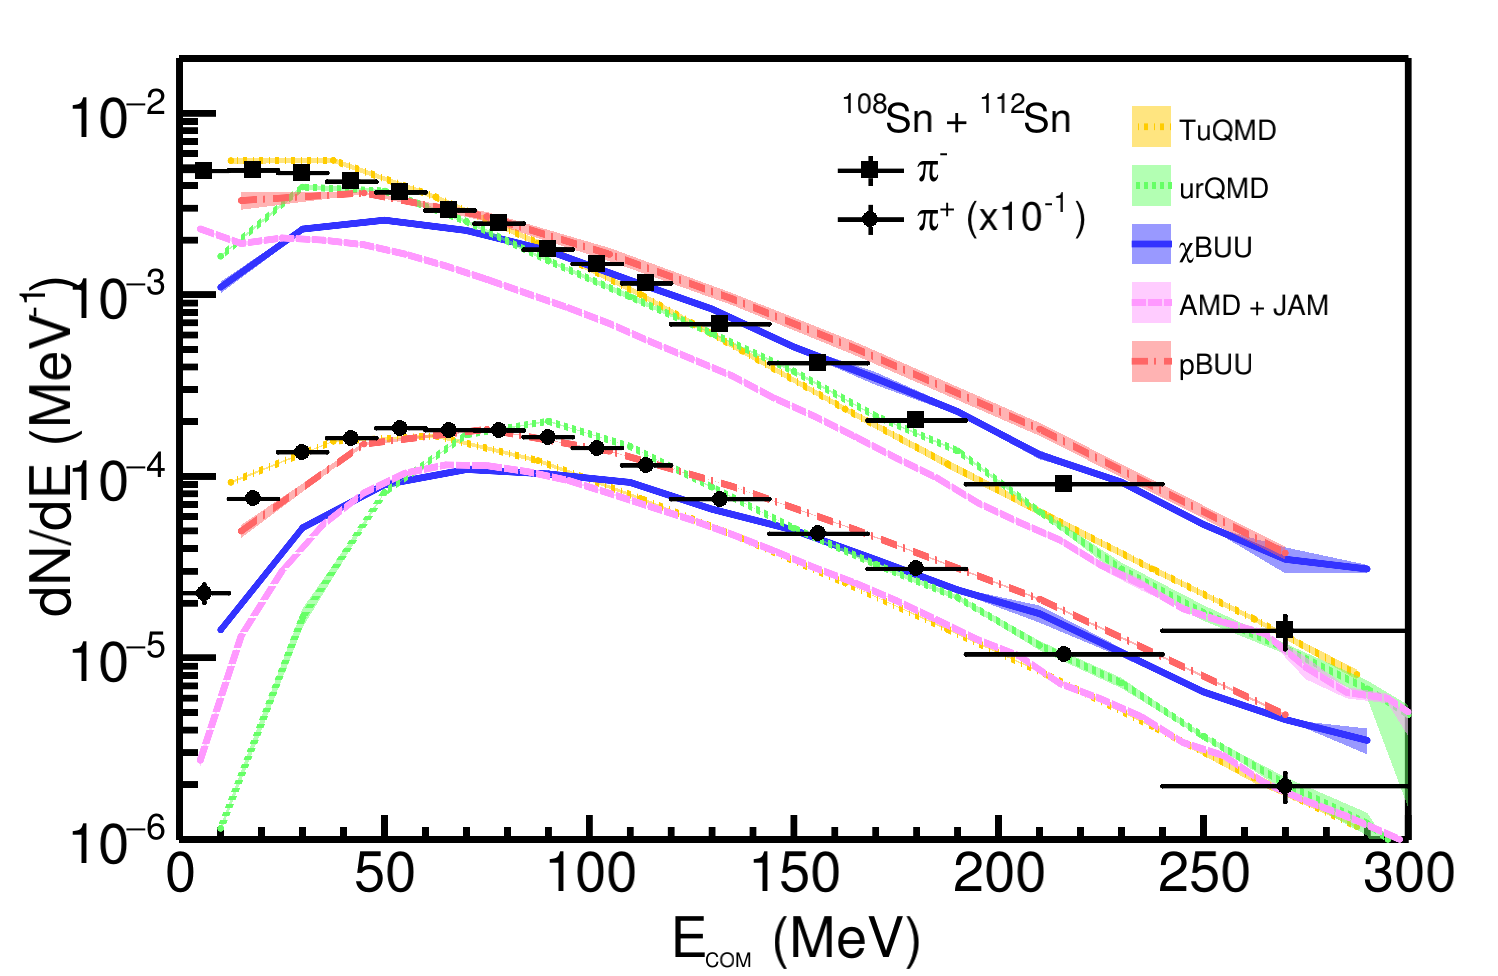
\includegraphics[width=\textwidth]{pionSpectra_sn108_sum.png}
\caption{Pion spectra $\tin{108}{112}$ system. }
\label{fig:pionspectraSn108}
\end{figure}


\begin{figure}[!htb]
\centering
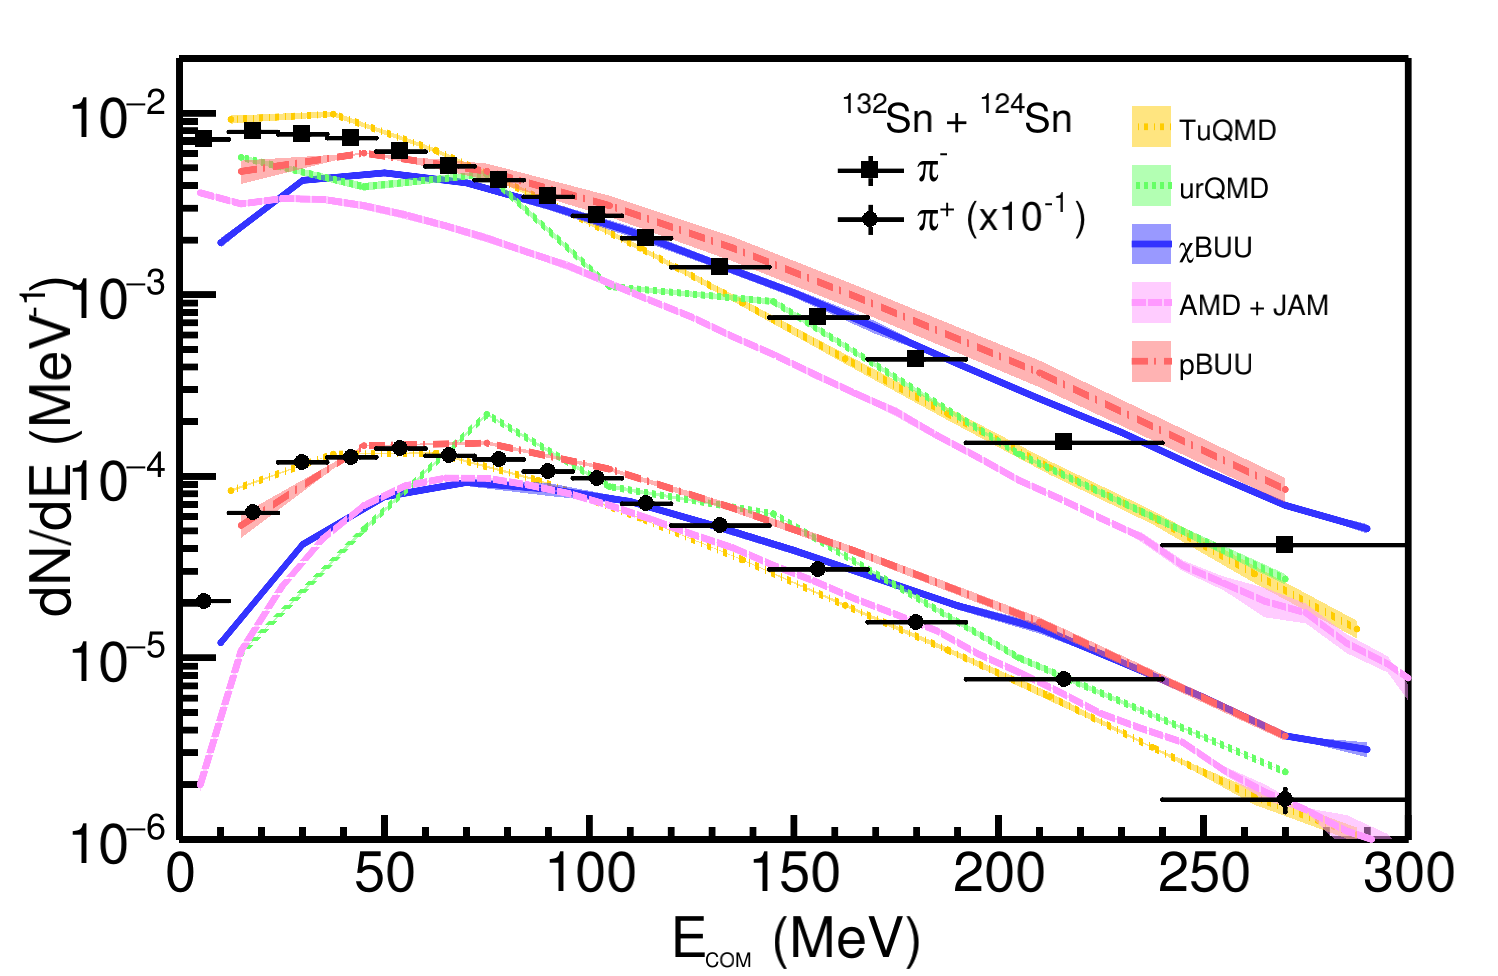
\includegraphics[width=\textwidth]{pionSpectra_sn132_sum.png}
\caption{Pion spectra $\tin{132}{124}$ system. }
\label{fig:pionspectraSn132}
\end{figure}


Figure~\ref{fig:pionspectra} shows pion CM kinetic energy spectra for both the $\tin{132}{124}$ and $\tin{108}{112}$ systems; corrected for efficiency and accounting for the solid angle of 4$\pi$. This data marks the first time pion spectral data has been measured at sub-threshold energies. In the pion spectra, we can see the effect of the coulomb potential, which accelerates $\pi^+$ and decelerates $\pi^-$ particles, due to the positive charge of the nuclear medium. The low $\pi^+$ production at low energy is caused by the coulomb barrier between protons which limits $\pi^+$ production at low energies. The Coulomb force has the largest effect on the spectra of the pions and will play an important role when observing the general shape of the pion spectral ratio. Besides the initial coulomb barrier for $\pi^+$ production, the coulomb force affects only the final energy of produced pions, and has almost no role in the total pion yield. 



%Add figure on Glauber model 
%Add figure on comparison to FOPI data









\section{Pion Spectral Ratio}


\begin{figure}[!htb]
\centering
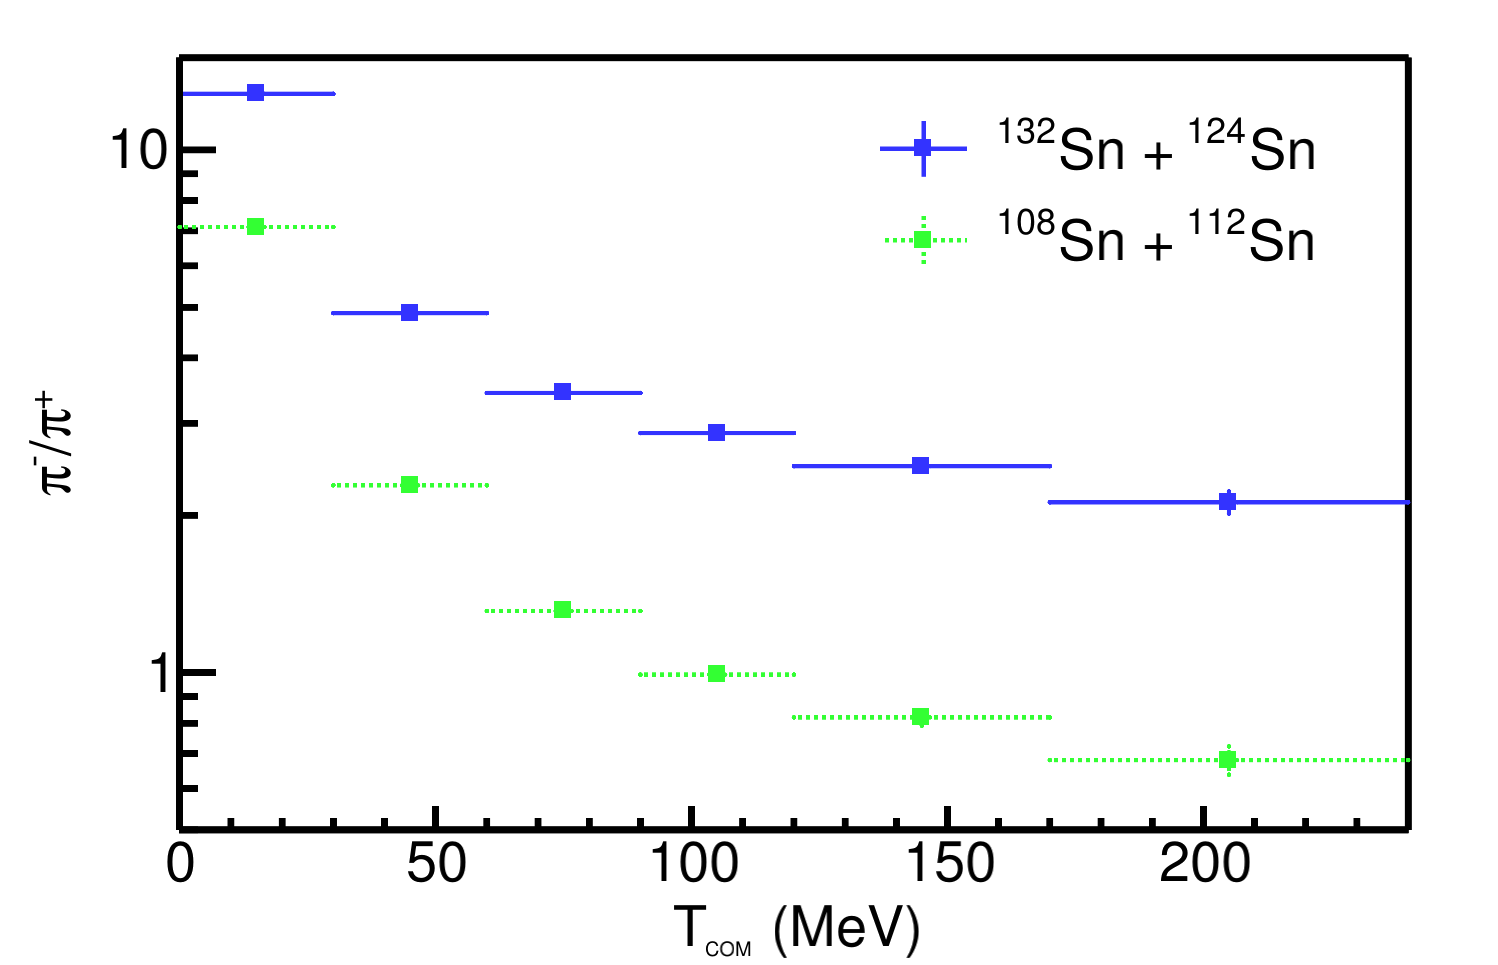
\includegraphics[width=\textwidth]{singleRatio.png}
\caption{Single ratio spectra}
\label{fig:SRspectra}
\end{figure}



\begin{figure}[!htb]
\centering
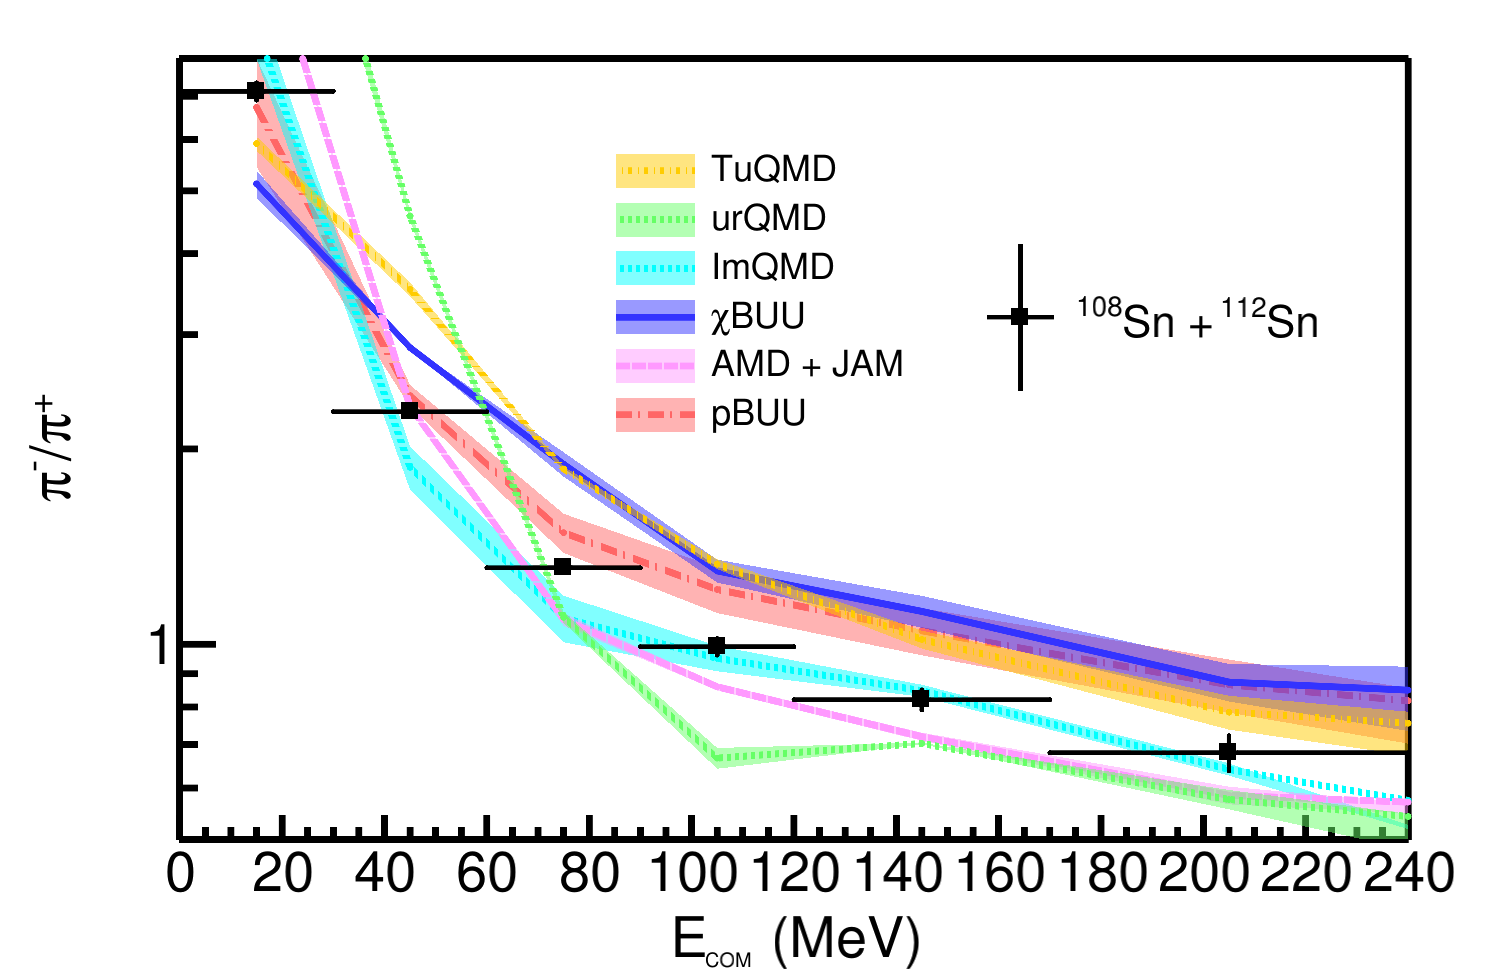
\includegraphics[width=\textwidth]{singleRatio108_log.png}
\caption{Single ratio $\tin{108}{112}$ system.}
\label{fig:SRsn108}
\end{figure}

\begin{figure}[!htb]
\centering
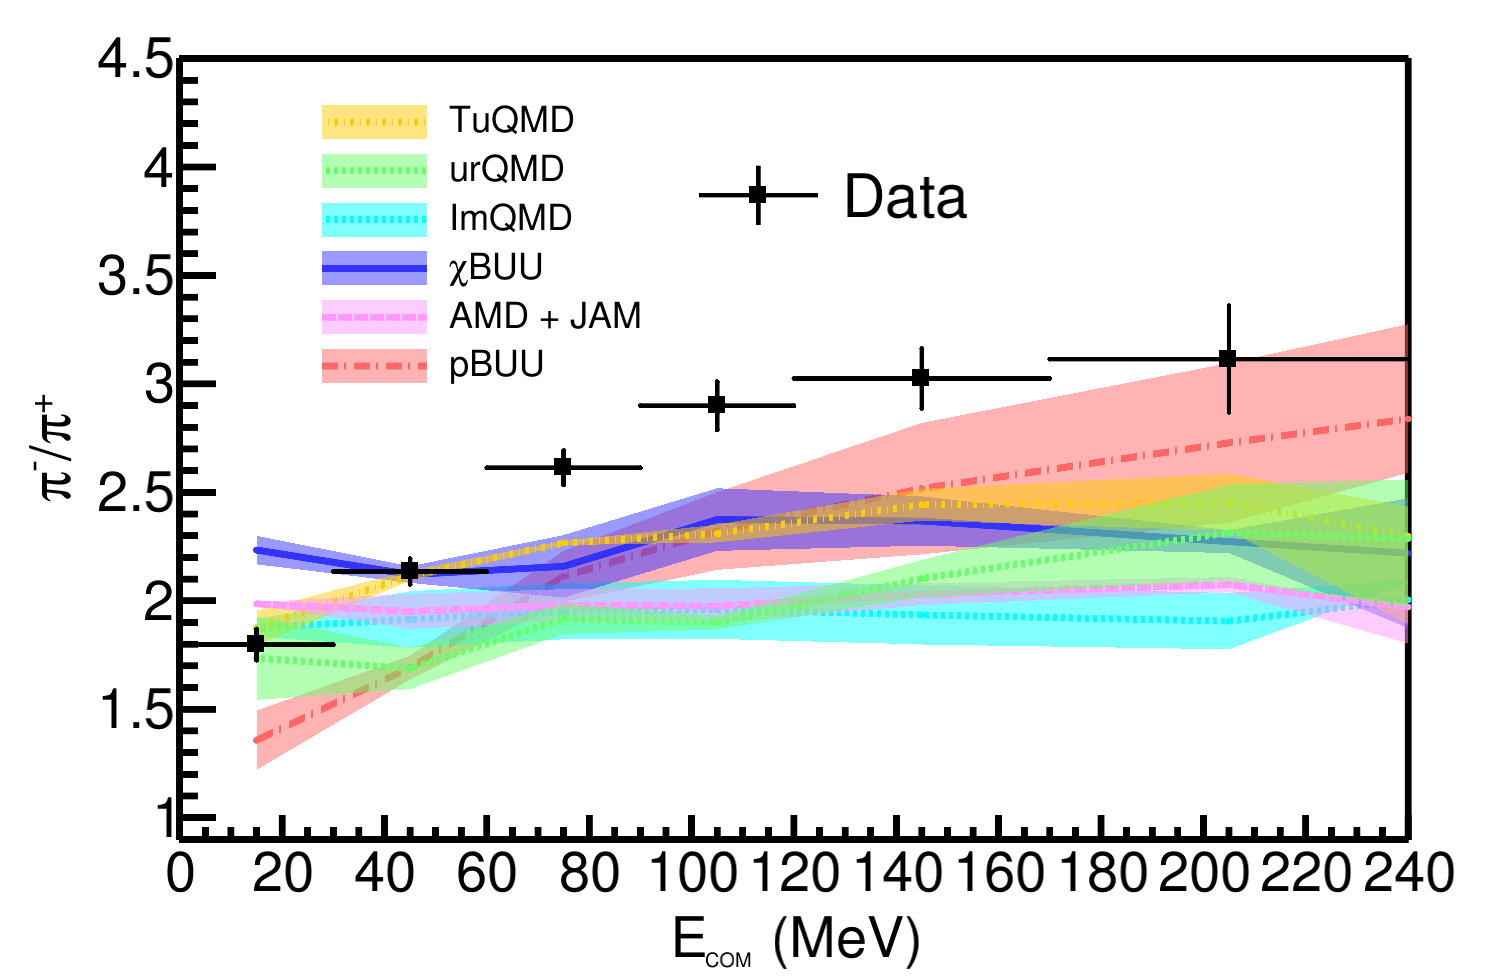
\includegraphics[width=\textwidth]{singleRatio132_sum.png}
\caption{Single ratio $\tin{132}{124}$ system.}
\label{fig:SRsn132}
\end{figure}

The pion spectral ratio is a rather promising observable. In particular, it may be more sensitive to the high density regions of the early collision. It is generally true, that high energy pions are more likely to exit the nuclear medium  earlier, and therefore be less prone to effects such as pion absorption and re-emission; all of which dilute the sensitivity of the pion observable to the high density behavior. Conversly, low energy pions are more likely to stay in the nuclear medium, and be affected by other effects such as the $\Delta$ potential in medium \cite{baoan_deltapotential}. Integrating these two regions to get the total pion yield dilutes the possible sensitivity the high energy pions have. Instead, we can construct the $Y(\pi^-)/Y(\pi^+)$ ratio as a function of the kinetic energy in the CM system with a particular focus on high energy pions.

%Mention and cite appendix for systematics

Figure~\ref{fig:SRspectra} shows the pion spectral ratio for both systems, which was measured with a high degree of efficiency and accuracy. The general hyperbolic shape arises from the Coulomb force on the two charged pion spectra mentioned earlier in Section~\ref{sec:pionSpectra}. Also notice the pion ratio is smaller for less neutron poor system, as we would expect since less neutron-neutron collisions produce less $\pi^-$. 



%Add figure of Theory for pion ratios

\section{Pion Double Ratio}
%Add figure of Theory for pion ratios

\begin{figure}[!htb]
\centering
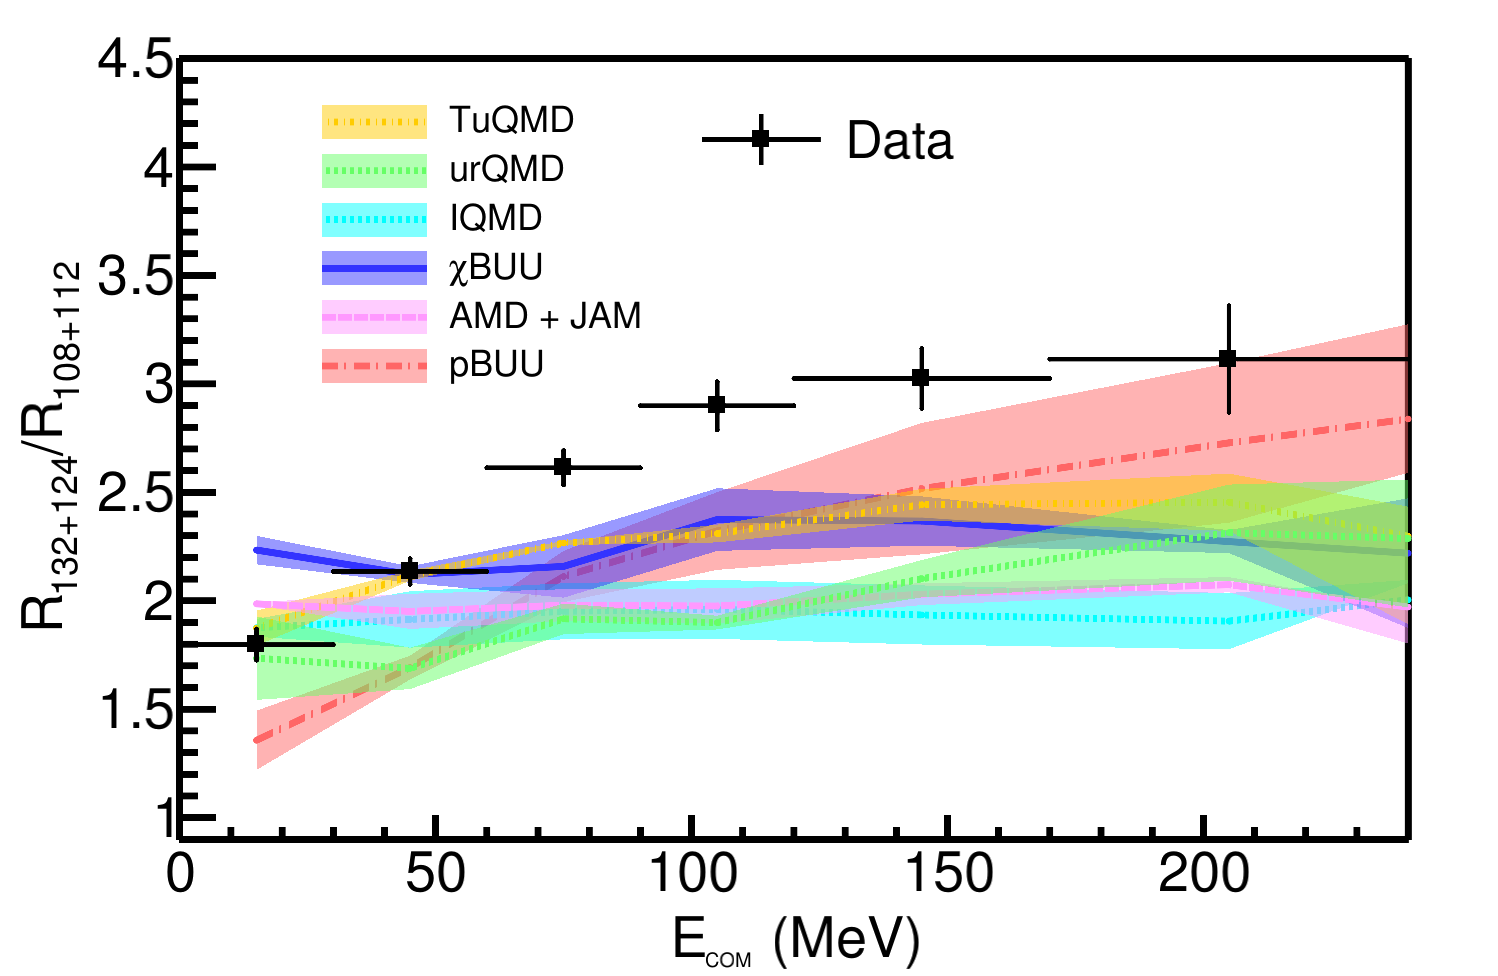
\includegraphics[width=\textwidth]{doubleRatio_sum.png}
\caption{}
\label{fig:spectraDR}
\end{figure}

In a similar way to the total pion double ratio, we can construct the spectral double ratio, the ratio between the two system's single ratios. In a similar way described in Section~\ref{sec:doubleRatio} we would expect systematic uncertainties in the experiment, and even in the theory --between the two systems-- to cancel out. For the same reasons as the pion spectral ratio, we would expect the high energy pions to be more sensitive to the high density region of the early collision. Here, just as in the total double ratio, the double ratio is significantly higher than any theory. Here as before, the bands in the theory represent the two extremes of the symmetry energy. 








